\documentclass[11pt,a4paper]{article}

% ===============================
% Packages
% ===============================
\usepackage[margin=2.2cm]{geometry}
\usepackage{setspace}
\usepackage{titlesec}
\usepackage{enumerate}
\usepackage{tabularx}
\usepackage{booktabs}
\usepackage{amsmath}
\usepackage{hyperref}
\usepackage{fancyhdr}
\usepackage{parskip}
\usepackage{lmodern}
\usepackage{xcolor}
\usepackage{environ}
\usepackage{verbatim}
\usepackage{tikz}
\usetikzlibrary{arrows.meta,positioning,calc,decorations.pathmorphing}

% ===============================
% Toggle: student vs instructor
% ===============================
\newif\ifsolutions
\solutionsfalse    % <-- Student version (no solutions)
%\solutionstrue       % <-- Instructor version (solutions visible)

% ===============================
% Styles (Style 1 — Clean Minimalist)
% ===============================
\definecolor{instrblue}{RGB}{0,70,160}
\definecolor{edgeblue}{RGB}{30,90,180}

% Diagram styles
\tikzset{
  read/.style={rectangle, rounded corners=2pt, draw=black!60, fill=black!5, inner sep=3pt, minimum width=18pt, minimum height=12pt, font=\footnotesize},
  node/.style={circle, draw=black!60, fill=black!5, inner sep=1.8pt, minimum size=16pt, font=\footnotesize},
  edge/.style={-Latex, very thin, draw=edgeblue},
  altedge/.style={-Latex, very thin, draw=black!60, dashed},
  pathhl/.style={-Latex, semithick, draw=black}, % highlight path (monochrome friendly)
  err/.style={-Latex, thin, draw=black, dashed}, % shows erroneous or low-confidence edges
  tip/.style={-Latex, thin, draw=black!60, densely dotted}
}

% ===============================
% Robust solution environment
% ===============================
\NewEnviron{solution}{%
  \ifsolutions
    \par\medskip
    \noindent\textbf{\color{instrblue}Solution. }\color{instrblue}\BODY
    \par\medskip\color{black}
  \fi
}

\newcommand{\instrnote}[1]{\ifsolutions{\color{instrblue}\emph{[#1]}}\fi}

% ===============================
% Header / Footer
% ===============================
\pagestyle{fancy}
\fancyhf{}
\lhead{Sequencing \& Assembly — Lecture 3}
\rhead{BINF301}
\rfoot{\thepage}
\ifsolutions
  \lhead{Instructor Version — Solutions Included}
\fi

% Section spacing
\titlespacing*{\section}{0pt}{10pt}{4pt}
\titlespacing*{\subsection}{0pt}{7pt}{3pt}

% ===============================
\begin{document}

\begin{center}
    {\LARGE \textbf{Lecture 3: Genome Assembly}}\\[6pt]
    {\Large \textbf{Student Handout \& In-Class Exercises}}\\[10pt]
    \textbf{Course:} BINF301 — Computational Biology \\
    \textbf{Instructor:} Tom Michoel \\
    \textbf{Date:} 21/01/2026\\
    \textbf{Created with Copilot}
\end{center}

\vspace{0.5cm}

% ----------------------------------------------------------
\section*{1. Overview}

This handout summarizes core ideas and adds inline diagrams:
\begin{itemize}
    \item What genome assembly is and why it is difficult.
    \item Two graph-based strategies: Overlap-Layout-Consensus (OLC) and De Bruijn Graphs (DBG).
    \item Complexity considerations.
    \item Handling errors and graph imperfections.
\end{itemize}

\instrnote{Slides referenced: OLC (5-12), DBG (13-25), non-perfect DBG (18), complexity (11, 19-25), error correction (27-38).}

% ----------------------------------------------------------
\section*{2. Genome Assembly Basics}

\subsection*{Definition \& Challenges}
\textbf{Genome assembly} combines sequencing reads into longer contiguous sequences (\emph{contigs}). Key challenges:
\begin{itemize}
    \item Repeats introduce ambiguity (multiple valid traversals).
    \item Sequencing errors introduce false paths/edges.
    \item Data volume drives graph size and cost.
\end{itemize}

% ----------------------------------------------------------
\section*{3. Overlap-Layout-Consensus (OLC)}

\noindent\textbf{Idea.} Reads are \emph{nodes}; overlaps are \emph{edges}. Reconstructing the genome corresponds (ideally) to a \textbf{Hamiltonian path} (visit each node/read once).

\begin{center}
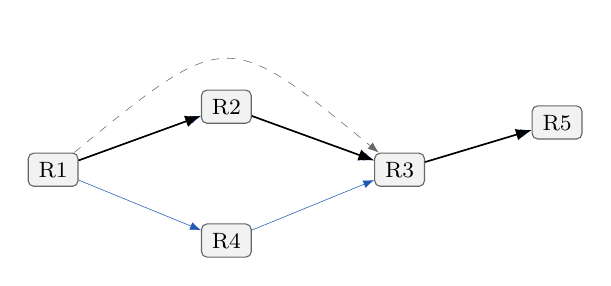
\begin{tikzpicture}[scale=1, every node/.append style={transform shape}]
  % Reads (nodes)
  \node[read] (R1) at (0,0) {R1};
  \node[read] (R2) at (2.2,0.8) {R2};
  \node[read] (R3) at (4.4,0) {R3};
  \node[read] (R4) at (2.2,-0.9) {R4};
  \node[read] (R5) at (6.4,0.6) {R5};

  % Overlap edges (solid = necessary; dashed = transitive)
  \draw[edge]   (R1) -- (R2);
  \draw[edge]   (R2) -- (R3);
  \draw[edge]   (R1) -- (R4);
  \draw[edge]   (R4) -- (R3);
  \draw[edge]   (R3) -- (R5);

  % A transitive edge (R1 -> R3) shown dashed
  \draw[altedge] (R1) .. controls (2.2,1.8) .. (R3);

  % Highlight one possible Hamiltonian-like path (illustrative)
  \draw[pathhl] (R1) -- (R2);
  \draw[pathhl] (R2) -- (R3);
  \draw[pathhl] (R3) -- (R5);
\end{tikzpicture}

\vspace{2mm}
\footnotesize OLC sketch: nodes are reads (R1--R5), edges show overlaps. Dashed edge indicates a \emph{transitive} overlap (can be removed).
\end{center}

\textbf{Why transitive reduction?} Removing transitive edges simplifies the graph and reduces ambiguity.

\begin{solution}
Nodes = reads; edges = overlaps. Transitive edges (e.g., R1$\to$R3 implied by R1$\to$R2 and R2$\to$R3) are redundant; removing them clarifies structure and helps with repeats.
\end{solution}

% ----------------------------------------------------------
\section*{4. De Bruijn Graphs (DBG)}

\noindent\textbf{Idea.} Nodes are \((k\!-\!1)\)-mers; edges are \(k\)-mers. Reconstruction corresponds to an \textbf{Eulerian path} (visit each edge once). Under perfect sequencing (each genomic \(k\)-mer present exactly once), the graph is Eulerian.

\begin{center}
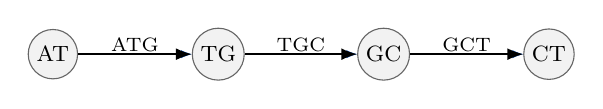
\begin{tikzpicture}[scale=1, every node/.append style={transform shape}]
  % (k-1)-mer nodes
  \node[node] (AT) at (0,0)   {AT};
  \node[node] (TG) at (2.1,0) {TG};
  \node[node] (GC) at (4.2,0) {GC};
  \node[node] (CT) at (6.3,0) {CT};

  % k-mer edges (solid)
  \draw[edge] (AT) -- node[above,sloped,inner sep=1pt]{\scriptsize ATG} (TG);
  \draw[edge] (TG) -- node[above,sloped,inner sep=1pt]{\scriptsize TGC} (GC);
  \draw[edge] (GC) -- node[above,sloped,inner sep=1pt]{\scriptsize GCT} (CT);

  % highlight Eulerian traversal (same as edges: monochrome safe)
  \draw[pathhl] (AT) -- (TG);
  \draw[pathhl] (TG) -- (GC);
  \draw[pathhl] (GC) -- (CT);
\end{tikzpicture}

\vspace{2mm}
\footnotesize DBG sketch: nodes are \((k\!-\!1)\)-mers, edges are \(k\)-mers; traversal uses each \emph{edge} exactly once (Eulerian).
\end{center}

\begin{solution}
OLC vs DBG: OLC seeks a Hamiltonian path over reads (NP-hard); DBG seeks an Eulerian path over edges (linear-time). DBG avoids explicit all-to-all overlaps by indexing \(k\)-mers.
\end{solution}

% ----------------------------------------------------------
\section*{5. Non-perfect Sequencing in DBG (errors/repeats)}

\noindent Errors, missing/duplicated \(k\)-mers create tips, bubbles, or spurious branches.

\begin{center}
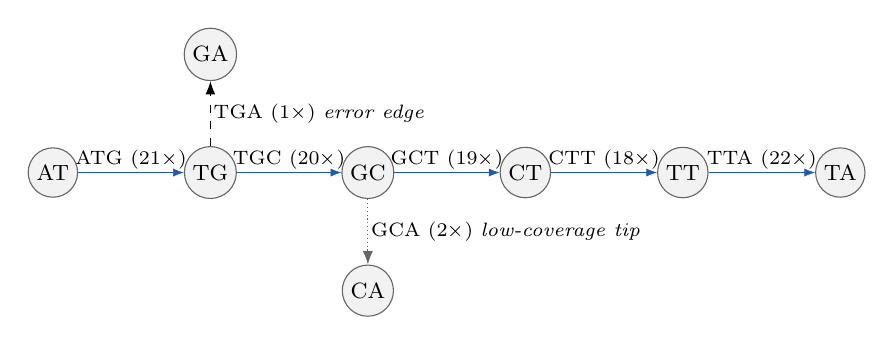
\begin{tikzpicture}[scale=1, every node/.append style={transform shape}]
  % True path nodes
  \node[node] (AT) at (0,0)   {AT};
  \node[node] (TG) at (2.0,0) {TG};
  \node[node] (GC) at (4.0,0) {GC};
  \node[node] (CT) at (6.0,0) {CT};
  \node[node] (TT) at (8.0,0) {TT};
  \node[node] (TA) at (10.0,0){TA};

  % True edges with frequencies
  \draw[edge] (AT) -- node[above,sloped,inner sep=1pt]{\scriptsize ATG (21×)} (TG);
  \draw[edge] (TG) -- node[above,sloped,inner sep=1pt]{\scriptsize TGC (20×)} (GC);
  \draw[edge] (GC) -- node[above,sloped,inner sep=1pt]{\scriptsize GCT (19×)} (CT);
  \draw[edge] (CT) -- node[above,sloped,inner sep=1pt]{\scriptsize CTT (18×)} (TT);
  \draw[edge] (TT) -- node[above,sloped,inner sep=1pt]{\scriptsize TTA (22×)} (TA);

  % Erroneous branch: TG -> GA
  \node[node] (GA) at (2.0,1.5) {GA};
  \draw[err] (TG) -- node[right,inner sep=1pt]{\scriptsize TGA (1×) \scriptsize \textit{error edge}} (GA);

  % Low-coverage tip: GC -> CA
  \node[node] (CA) at (4.0,-1.5) {CA};
  \draw[tip] (GC) -- node[right,inner sep=1pt]{\scriptsize GCA (2×) \scriptsize \textit{low-coverage tip}} (CA);

\end{tikzpicture}

\vspace{2mm}
\footnotesize
Non-perfect DBG.  
Top chain: high-frequency true k-mers (18–22×).  
Dashed branch: \textit{TGA} (1×) is a sequencing error → novel, unsupported k-mer.  
Dotted tip: \textit{GCA} (2×) may be real but insufficiently sampled → low-coverage artifact.
\end{center}



\begin{solution}
High coverage: true edges occur many times; erroneous edges are low-frequency and can be removed. Tip/bubble removal simplifies the graph.
\end{solution}

% ----------------------------------------------------------
\section*{6. Complexity (OLC vs DBG)}

\noindent \textbf{OLC.} Building overlap graphs can be \(O(N^2)\) in reads; graph can be large (especially for short reads).  
\noindent \textbf{DBG.} Construction scales with number of \(k\)-mers (\(\approx O(N)\)); more memory-efficient for high read counts, but sacrifices long-read continuity.

% % Tiny schematic: “many short reads → OLC heavy” vs “DBG compacts k-mers”
% \begin{center}
% \begin{tikzpicture}[scale=1, every node/.append style={transform shape}]
%   % OLC side
%   \node at (0,1.3) {\footnotesize OLC (short reads)};
%   \foreach \i in {0,...,7}{
%     \node[read, minimum width=12mm] (S\i) at (\i*0.9-3.,0.6) {};
%   }
%   \foreach \i in {0,...,6}{
%     \draw[edge] (S\i) -- (S\the\numexpr\i+1\relax);
%   }

%   % DBG side
%   \node at (7.8,1.3) {\footnotesize DBG (k-mer compaction)};
%   \node[node] (n1) at (6.2,0.6) {AA};
%   \node[node] (n2) at (7.6,0.6) {AT};
%   \node[node] (n3) at (9.0,0.6) {TT};
%   \draw[edge] (n1) -- node[above,sloped,inner sep=1pt]{\scriptsize AAT} (n2);
%   \draw[edge] (n2) -- node[above,sloped,inner sep=1pt]{\scriptsize ATT} (n3);
% \end{tikzpicture}
% \end{center}

\newpage
% ----------------------------------------------------------
\section*{7. In-Class Exercises}

\subsection*{Exercise 1 — Understanding OLC Overlap Graphs}
Using OLC diagrams:
\begin{itemize}
    \item Identify nodes vs edges.
    \item Find transitive edges (and say why to remove them).
\end{itemize}

\begin{solution}
Nodes = reads; edges = overlaps. Transitive edges are redundant (e.g., R1$\to$R3 implied by R1$\to$R2 and R2$\to$R3). Removing them clarifies true structure.
\end{solution}

% -------------------------------
\subsection*{Exercise 2 — Hamiltonian vs Eulerian}
Reads: \verb|ACTTTCTTCTGG|.  
\begin{itemize}
    \item In OLC: visit each \emph{read} once (Hamiltonian).
    \item In DBG: traverse each \emph{edge} once (Eulerian).
    \item Why is one NP-hard and the other linear-time?
\end{itemize}

\begin{solution}
OLC’s Hamiltonian path problem is NP-hard; DBG’s Eulerian path is linear-time. DBG avoids exhaustive overlap detection by working with \(k\)-mers.
\end{solution}

% -------------------------------
\subsection*{Exercise 3 — DBG Error Scenario}
Genome: \verb|ATGCTTA|  
Reads (\(k=3\)): \verb|ATG, TGC, GCT, CTT, TTA, TGA| (\emph{TGA} erroneous)

Tasks:
\begin{itemize}
    \item Build the 3-mer DBG (nodes=2-mers; edges=3-mers).
    \item Identify the inconsistent edge.
    \item Explain coverage-based pruning.
\end{itemize}

\begin{solution}
Erroneous edge: \emph{TGA} (TG$\to$GA) forms a branch not on the main path. High coverage → true edges dominate counts; low-frequency error edges are pruned.
\end{solution}

% -------------------------------
\subsection*{Exercise 4 — Choosing OLC vs DBG}
\begin{itemize}
    \item Why OLC for long reads and DBG for short reads?
\end{itemize}

\begin{solution}
Long reads reduce the number of nodes; overlaps are manageable \(\Rightarrow\) OLC good. Short reads produce massive graphs \(\Rightarrow\) OLC heavy; DBG compacts data into \(k\)-mers efficiently.
\end{solution}

% ----------------------------------------------------------
\end{document}